\chapter{Dark matter interpretations of Run 1 searches for invisibly decaying Higgs bosons}
\label{chap:interp}
As well as combining the results of the \ac{VBF} searches with other channels, it is also possible to interpret them as limits on other specific models. Interpretations of the \ac{VBF} search results in several \ac{DM} models are described in \SectionRef{sec:dminterp}.

%??CHECK PLOT AXIS LABEL SIZES AND THAT LEGEND TERMS ARE STANDARD OR IN TEXT

\section{Simulation Techniques and Validation}
\label{sec:dmval}

%??start with internal sample
%??validate against powheg plus delphes: when generated with same PU etc. found to agree to within 10%
%??validate powheg plus delphes against mg plus delphes table from phenoplots281015.pdf
\begin{table}
  \caption{}%??
  \label{tab:mgvspowhegdelphes}
  \begin{tabular}{lcc}
    \hline
    \hline
    
    \hline

    \hline
    \hline
  \end{tabular}
\end{table}

%??recreation of metsig and l1met
%??systematic scaling


\begin{figure}
  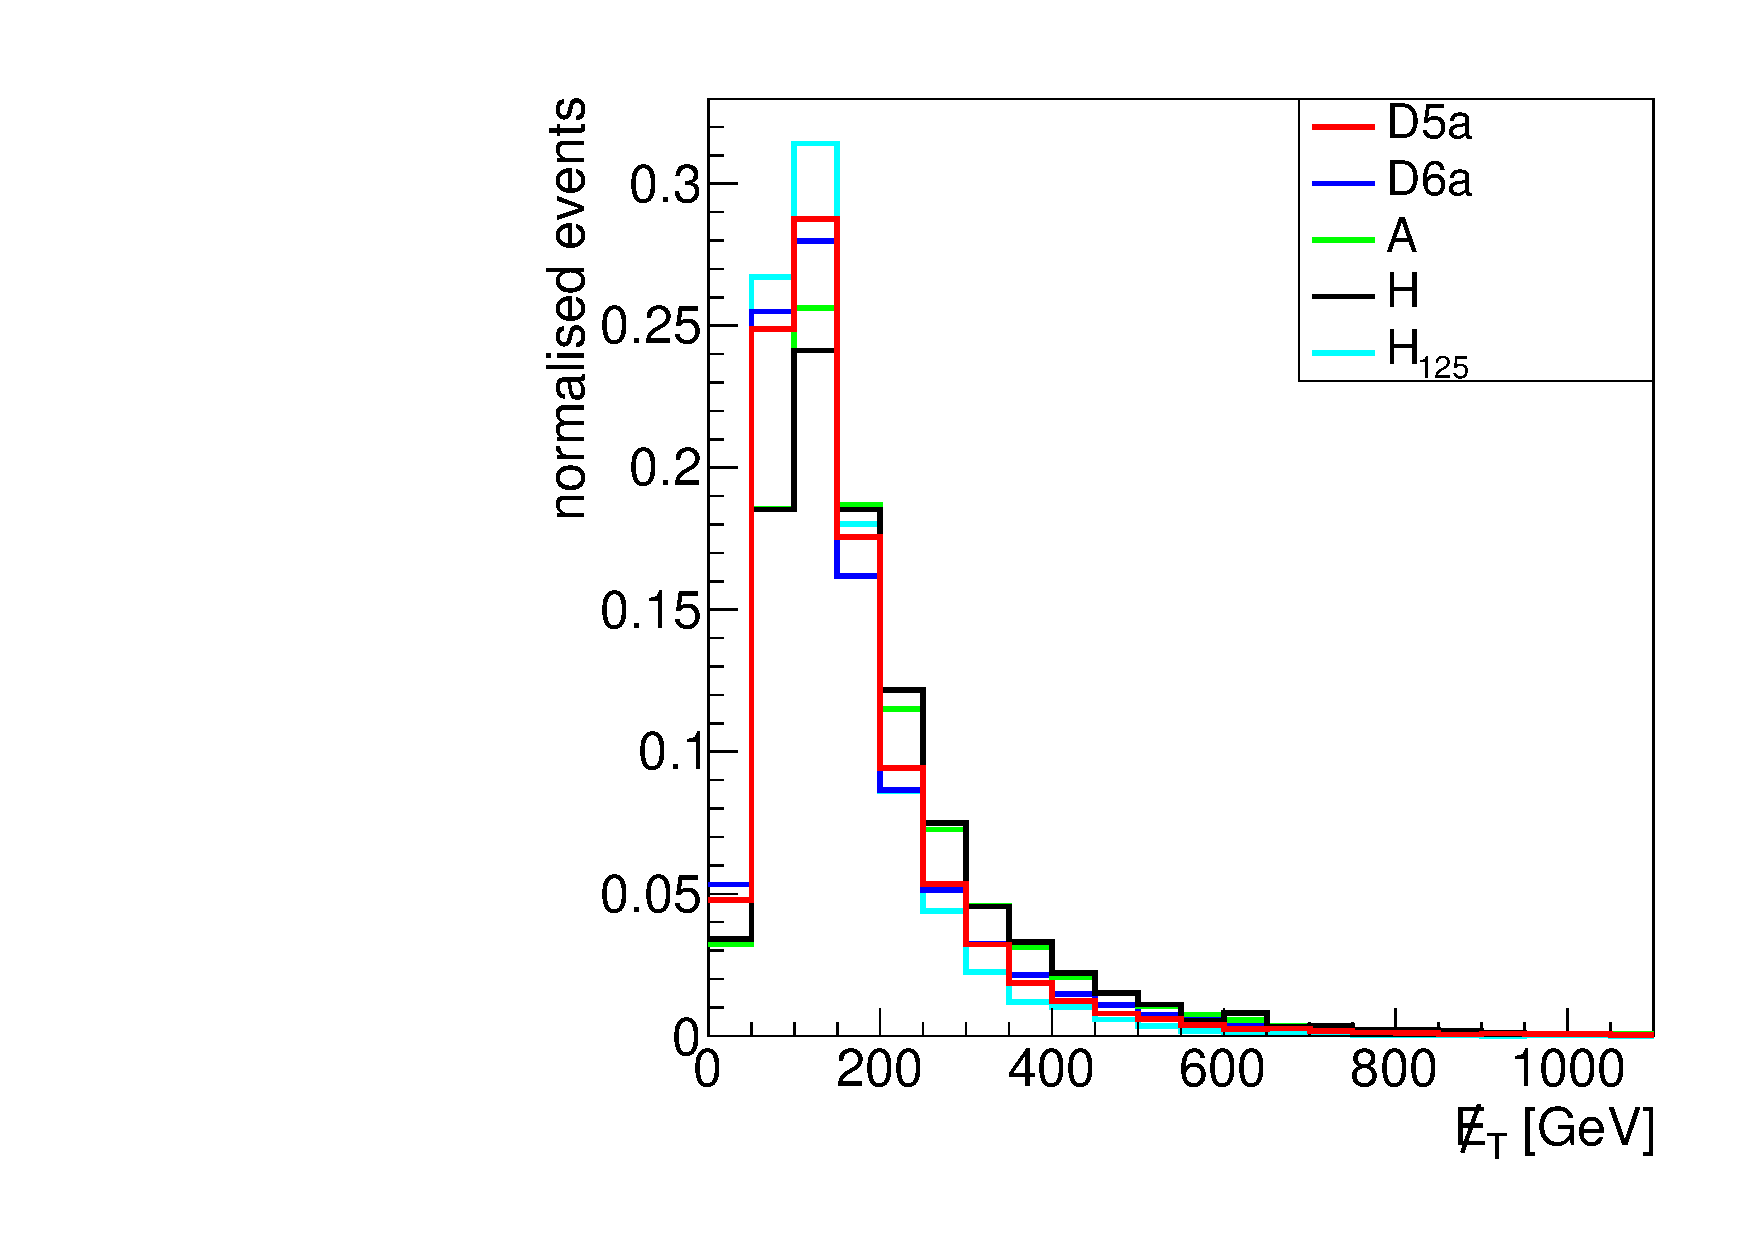
\includegraphics[width=.65\largefigwidth]{plots/interp/modelmet.pdf}
  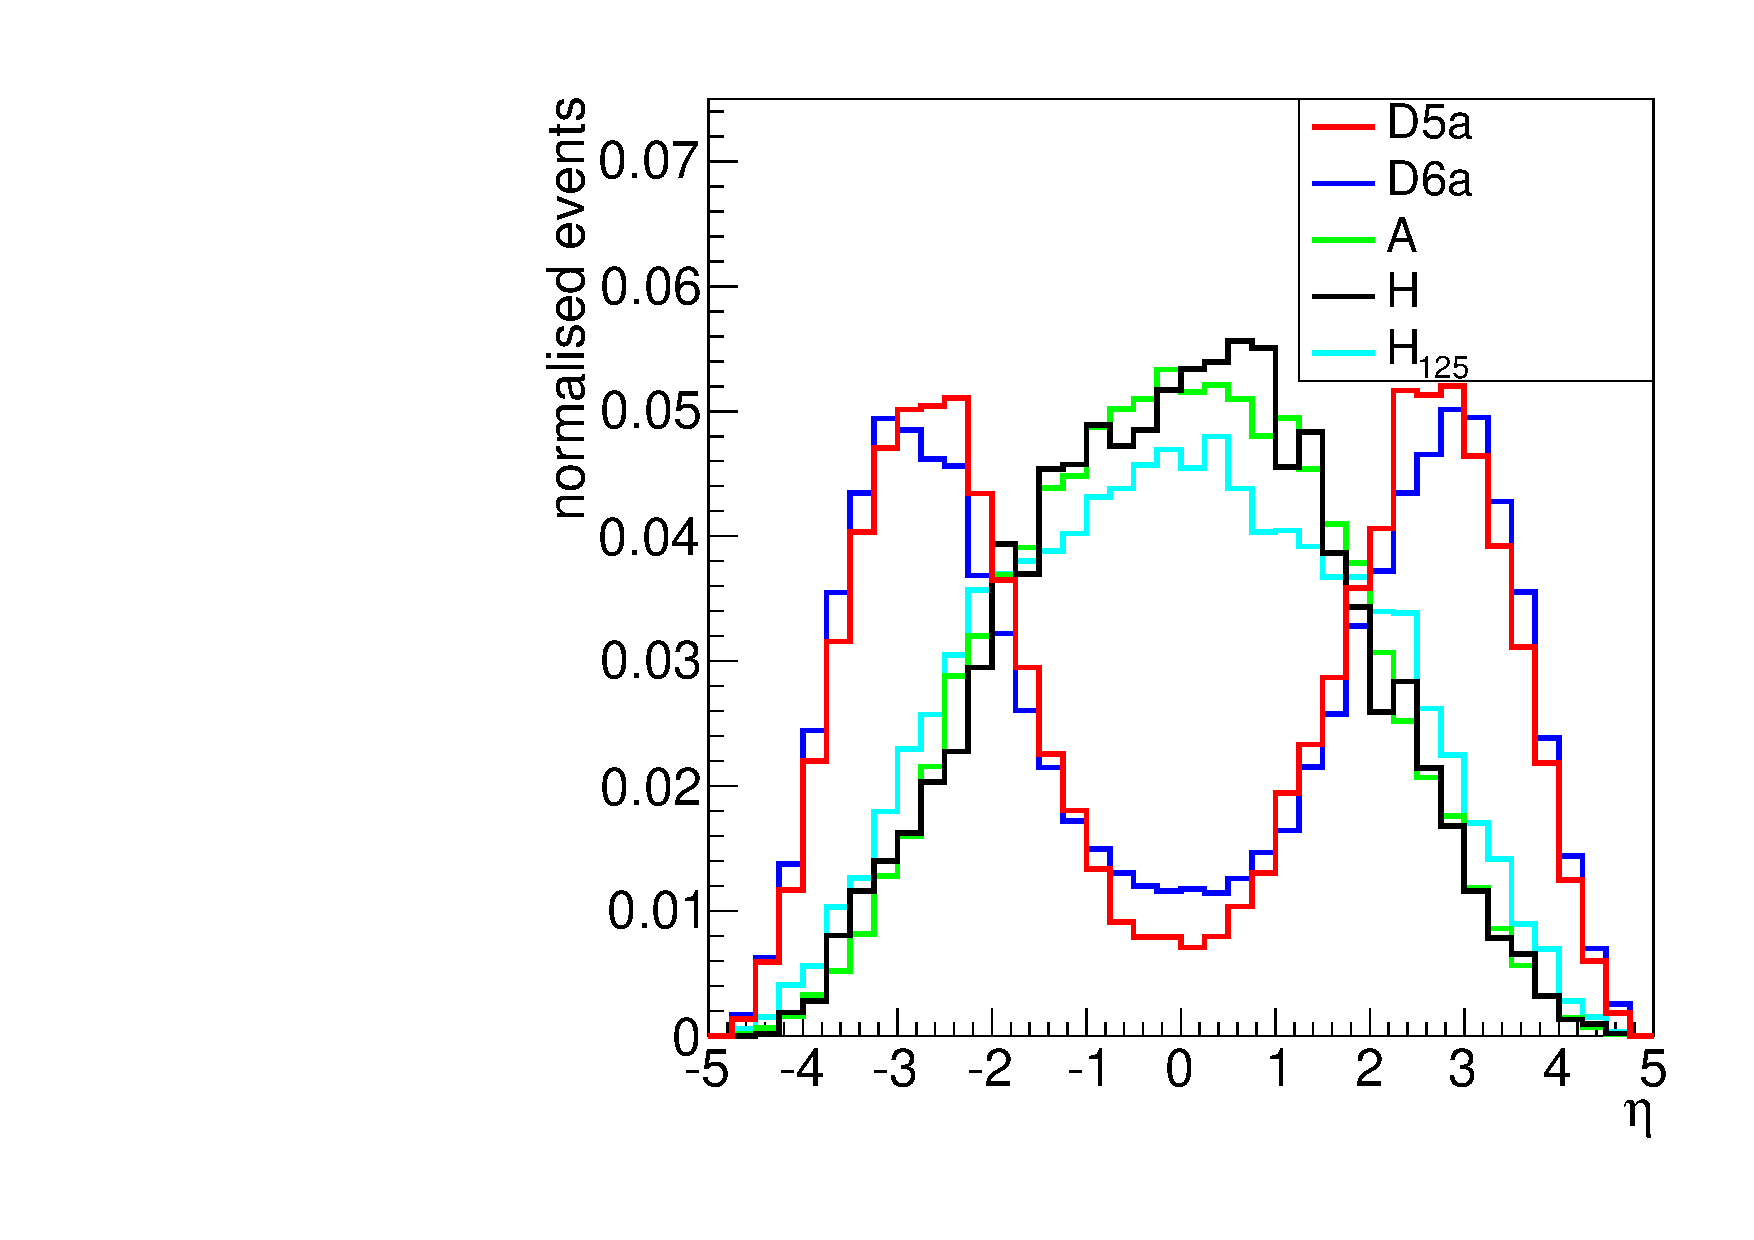
\includegraphics[width=.65\largefigwidth]{plots/interp/modeleta.pdf}
  \caption{}%??
  \label{fig:dmmodelkinematics}
\end{figure}

\section{Results}
\label{sec:dmresults}

\begin{figure}
  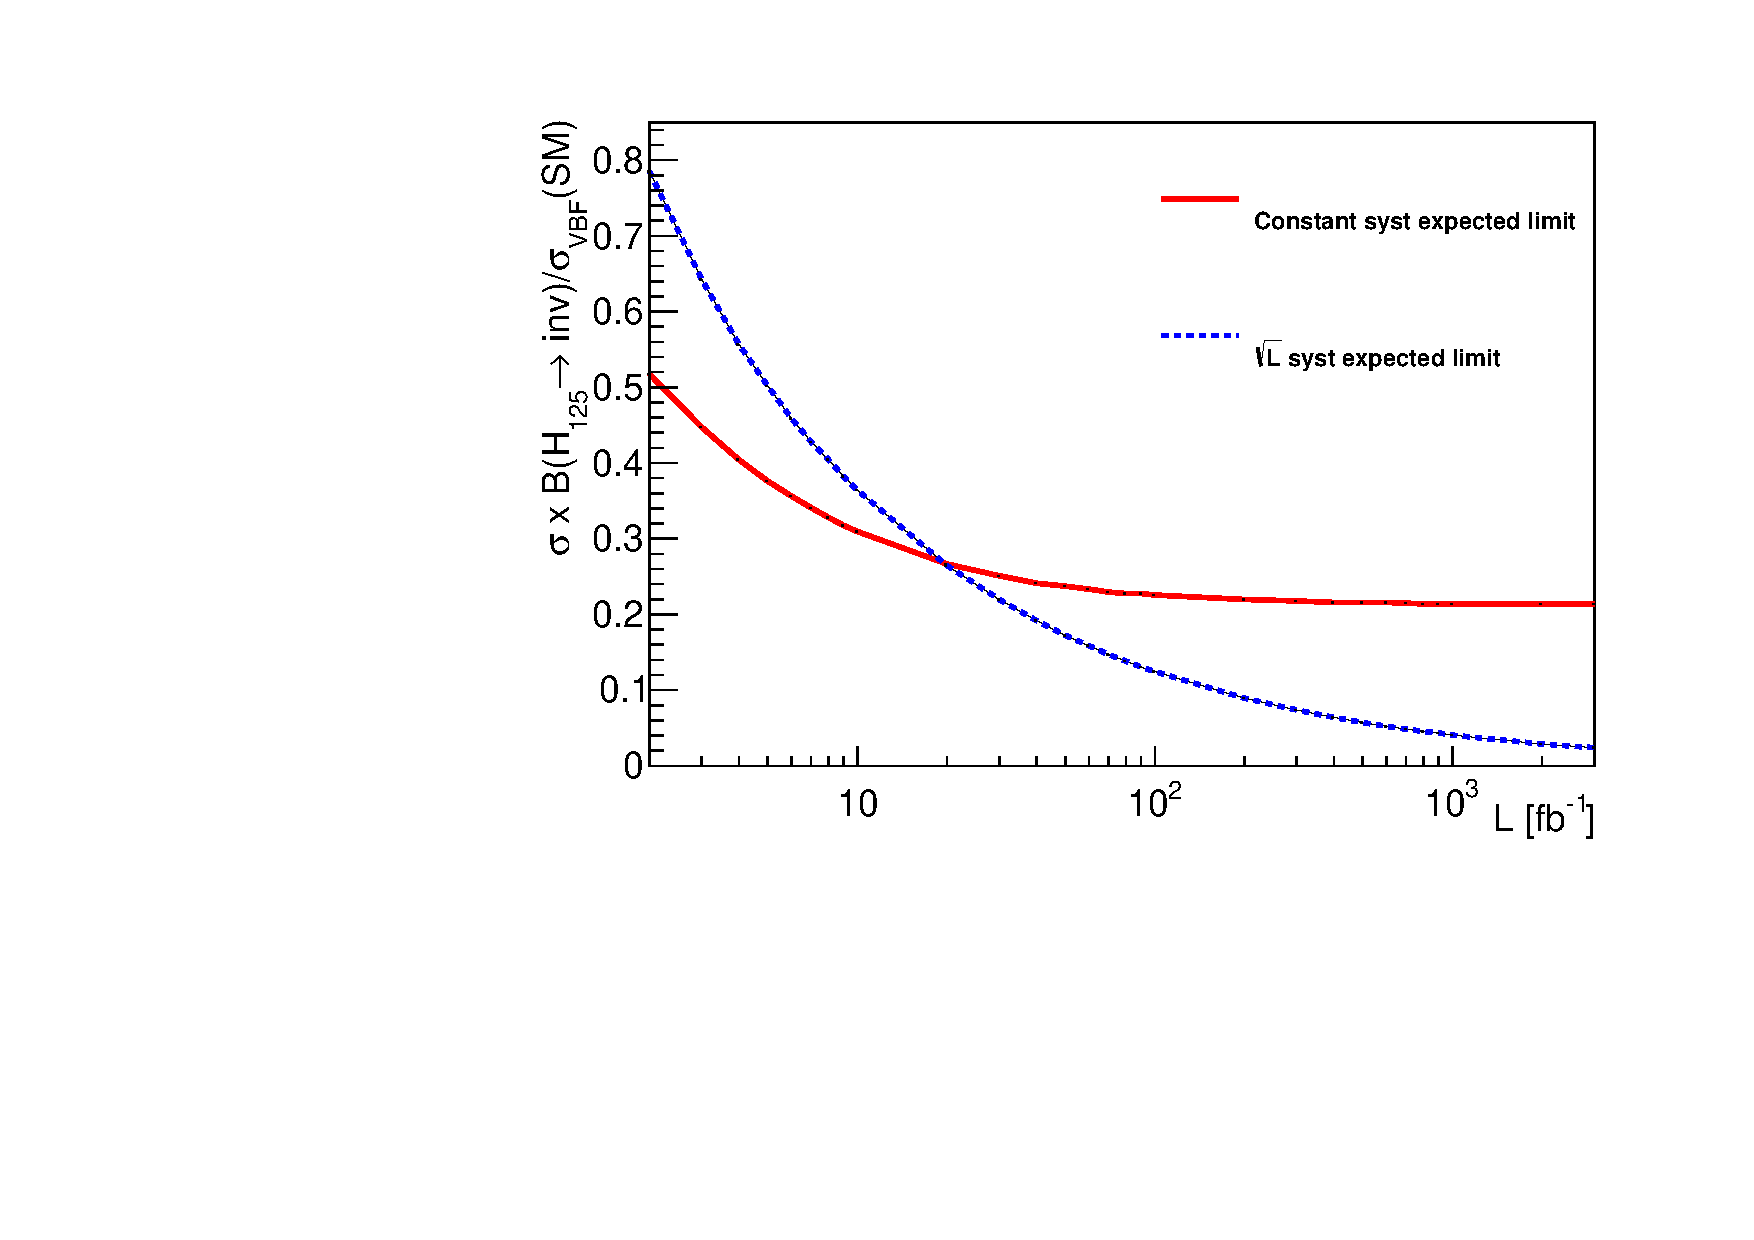
\includegraphics[width=.65\largefigwidth]{plots/interp/phenoprojectedvbflimit.pdf}
  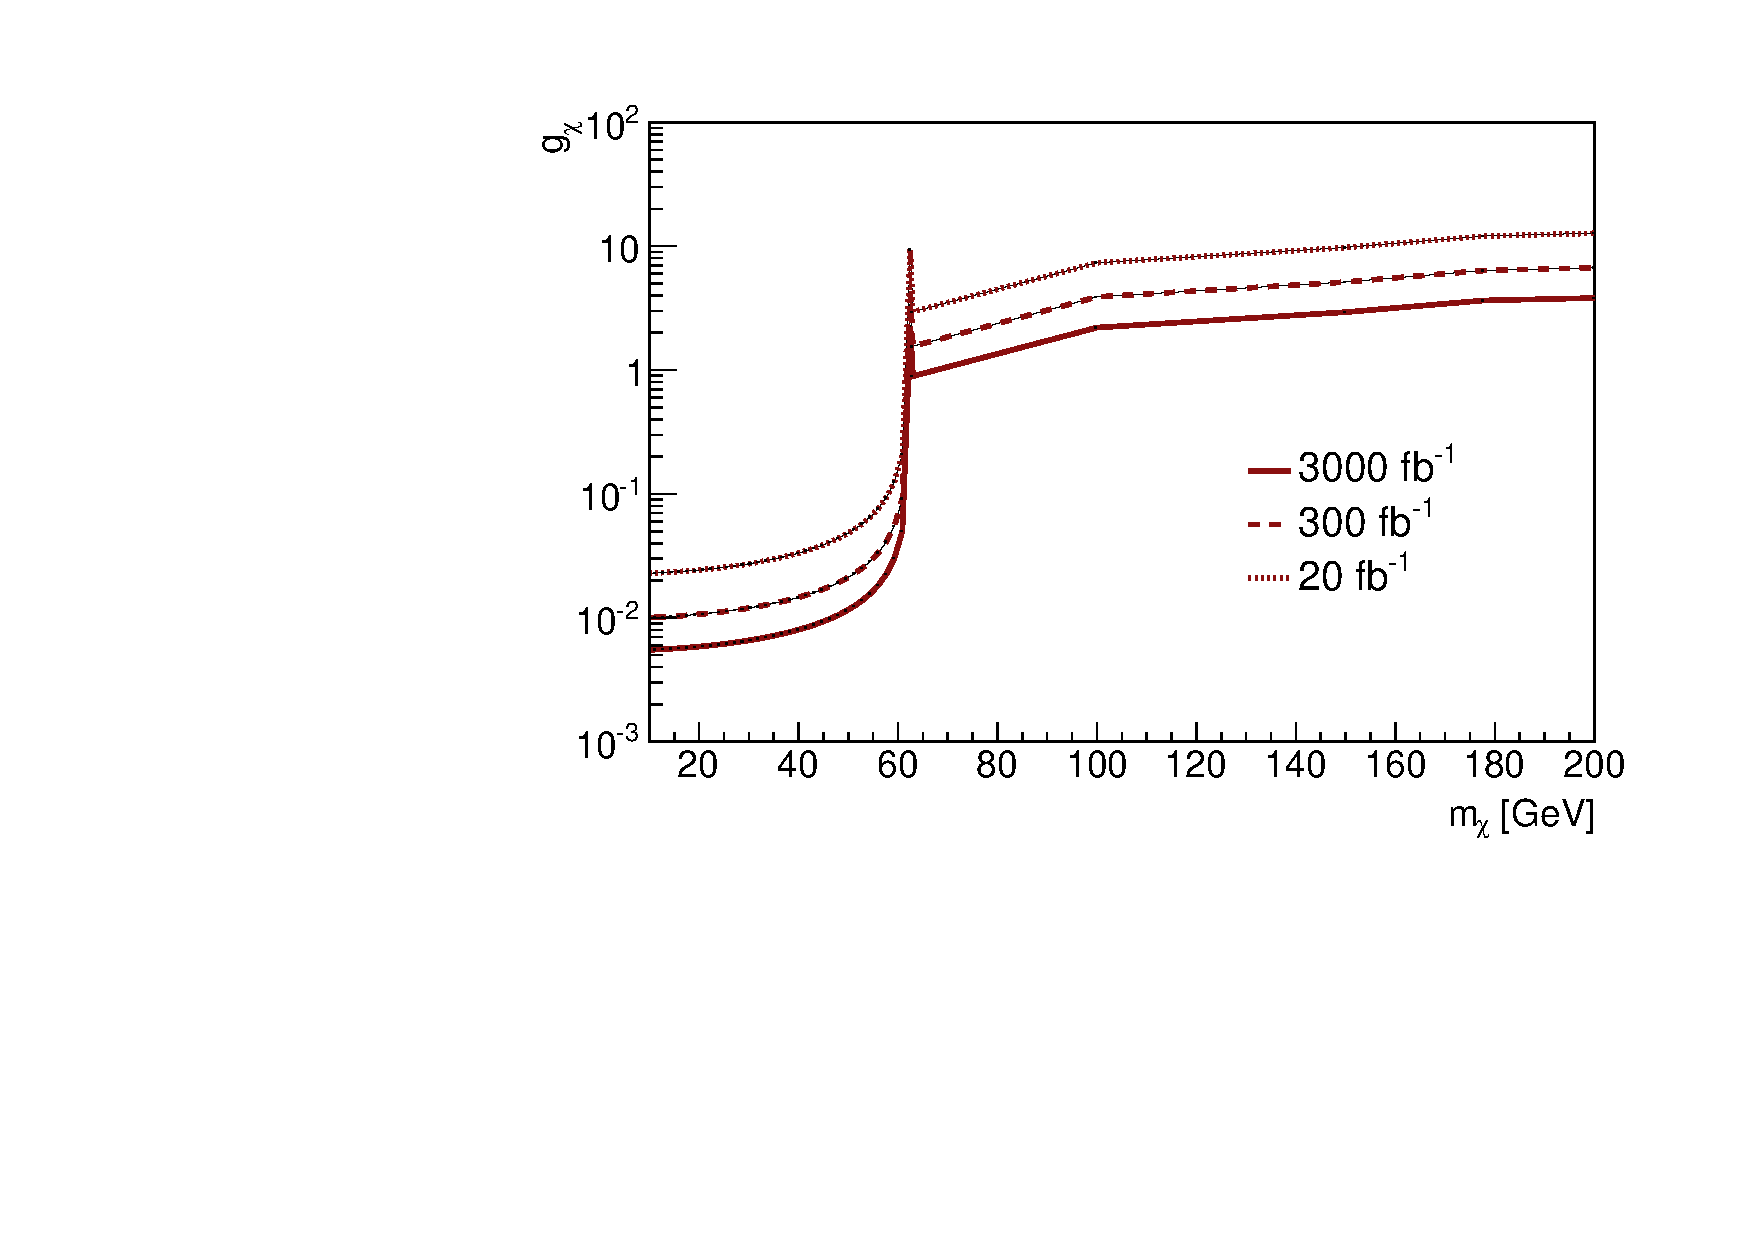
\includegraphics[width=.65\largefigwidth]{plots/interp/125higgsgchilimit.pdf}
  \caption{}%??
  \label{fig:smprojectedlimits}
\end{figure}
